\documentclass{article}

% Langue
\usepackage[utf8]{inputenc}
\usepackage[T1]{fontenc}      
\usepackage[francais]{babel}

% Mise en forme générale
\usepackage[top=2.5cm,bottom=2.5cm,right=2.5cm,left=2.5cm]{geometry}

% Package divers
\usepackage{chemist} 
\usepackage[version=3]{mhchem}
\usepackage{chemfig}
\usepackage[squaren, Gray]{SIunits}
\usepackage{sistyle}
\usepackage[autolanguage]{numprint}
\usepackage{url}
\usepackage{rotating}
\usepackage{xcolor,colortbl}
\definecolor{Gray}{gray}{0.85}

\usepackage{hyperref}
\hypersetup{
    colorlinks,
    citecolor=black,
    filecolor=black,
    linkcolor=black,
    urlcolor=black
}

% Nouvelles commandes
\newcommand{\std}{\ensuremath{^{\circ}}}
\newcommand\ph{\ensuremath{\mathrm{pH}}}
\newcommand{\annexe}{\part{Annexes}\appendix}
\newcommand{\biblio}[1]{\bibliographystyle{plain}\bibliography{#1}\nocite{*}}

\newcommand{\doctitle}[1]{
	\title{#1}
	\author{\textbf{Groupe 124.3}\\
	\textsc{Frenyo} Péter (6266-12-00)\\
	\textsc{Gillain} Nathan (7879-12-00)\\
	\textsc{Lamine} Guillaume (7109-13-00)\\
	\textsc{Piraux} Pauline (2520-13-00)\\
	\textsc{Paris} Antoine (3158-13-00)\\
	\textsc{Quiriny} Simon (4235-13-00)\\
	\textsc{Schrurs} Sébastien (7978-13-00)}
	\date{\today}

	\begin{document}

	\maketitle
	\tableofcontents
}

\doctitle{Projet 3 - Synthèse}
\newpage
\section{Thermochimie}
\subsection{Notion d'équilibre réactionnel}
Soit une réaction chimique quelconque
\begin{chemmath}
	lL + mM  \Leftrightarrow xX + yY.
\end{chemmath}
Pour cette réaction, on peut écrire un
degré d'avancement $\xi(t)$ défini comme
suit
\[ \xi(t) = \frac{n_X(t) - n_{X0}}{x} =
\frac{n_Y(t) - n_{Y0}}{y} = \frac{n_L0 - n_{L}(t)}{l}
= \frac{n_M0 - n_{M}(t)}{m}. \]
Une réaction est spontanée si sa variation
d'enthalpie libre est négative 
\[ \frac{\mathrm{d}G}{\mathrm{d}\xi}(\xi) < 0. \]
A l'équilibre on aura 
\[ \frac{\mathrm{d}G}{\mathrm{d}\xi}(\xi_{eq}) = 0.\]
Or, on sait (cfr. cours de thermodynamique de première) que
\[ \frac{\mathrm{d}G}{\mathrm{d}\xi} = \Delta G^{\circ}(T)
+ RT\ln{Q_r(\xi,p,T)}\]
où $Q_r(\xi,p,T)$, le quotient réactionnel, est
défini en fonction des activités des composés
\[ Q_r(\xi,p,T) = \frac{(a_X(\xi))^x(a_Y(\xi))^y}{(a_L(\xi))^l(a_M(\xi))^m}. \]
Pour rappel, les activités dépendant de la phase
de l'élement :
\begin{itemize}
	\item Solides et liquides pures : $a=1$ ;
	\item Gaz : $a = \frac{p}{p^{\circ}}$ avec
	$p^{\circ} = \unit{1}{\bbar}$ la pression standard ;
	\item Solutions aqueuses : $a = \frac{c}{c^{\circ}}$
	avec $c^{\circ} = \unit{1}{\mole\per\liter}$ la concentration
	standard.
\end{itemize}
On définit enfin la constante d'équilibre 
\[ K(t) = Q_r(\xi_{eq}) = \exp{-\frac{\Delta G^{\circ}(T)}{RT}}. \]

\subsection{Notion d'enthalpie de réaction}
Pour la même réaction quelconque que dans la section
précédente, on définit l'enthalpie de réaction
\[ \Delta H\std = x\Delta H\std_{form,X} + y\Delta H\std_{form,Y}
- l\Delta H\std_{form,Y} - m\Delta H\std_{form,M}.\]
Cette enthalpie, qui correspond à la chaleur de réaction 
est souvent exprimée en \unit{}{\joule\per\kilo\gram}
ou en \unit{}{\joule\per\mole} d'un composé présent en quantité
stoéchiométrique égale à 1. Si l'enthalpie de réaction est négative,
alors ça correspond à de la chaleur dégagée par le
système, la réaction est alors exothermique. Si au contraire
elle est positive, ça correspond à de la chaleur absorbée
par le système, la réaction est alors entothermique.

\paragraph{Influence de la température} L'enthalpie
varie avec la température
\[ \Delta H\std(T_2) = \Delta H\std(T_{ref})
+ \int_{T_1}^{T_2} \Delta C_p \mathrm{d}T \]
où $\Delta C_p$ est la différences des capacités
calorifiques molaires des produits et des réactifs
pondérées par leur coefficient stoéchiométrique.
\paragraph{Influence de la pression} L'enthalpie
ne dépend pas de la pression.

% TODO : ajouter entropie et enthalpie de libre comme
% c'est quand même utilisé dans le projet pour calculer
% les constantes d'équilibre.

\subsection{Calcul d'un équilibre global pour plusieurs réactions simultanées
(comme dans le réformeur primaire)}
Dans le réformeur primaire, nous avons dans un premier temps
calculer les constantes d'équilibre $K_1$ et $K_2$ des deux 
réactions à partir de l'enthalpie libre. Nous avons ensuite
dressé deux tableaux d'avancement.

	\begin{table}[ht!]
		\centering
		\begin{tabular}{c|cccccccc}
									& \ce{CH_4(g)} 				&+& \ce{H_2O(g)} 			 	&	$\Leftrightarrow$ 		& \ce{CO(g)} 			&+& \ce{3H_2(g)} \\
			\hline
			$n_i$ 			& $n_{01}$ 						& & $n_{02}$						& 											& 0								&	& 0 \\
			$n_{eq}(x)$	&	$n_{01}-x$ 					& & $n_{02}-x-y$				& 											& $x-y$ 					&	& $3x+y$ \\
			\hline 
			$a_{eq}$		& $\frac{n_{01}-x}{n_{gaz,tot}}\frac{p}{p\std}$ &
																				& $\frac{n_{02}-x-y}{n_{gaz,tot}}\frac{p}{p\std}$ &
																															& $\frac{x-y}{n_{gaz,tot}}\frac{p}{p\std}$ &
																																									& $\frac{3x+y}{n_{gaz,tot}}\frac{p}{p\std}$
		\end{tabular}
		\caption{Tableau d'avancement de la première réaction.}
		\label{avancement1}
	\end{table}
	
	\begin{table}[ht!]
		\centering
		\begin{tabular}{c|cccccccc}
									& \ce{CO(g)} 				&+& \ce{H_2O(g)} 			 		&	$\Leftrightarrow$ 		& \ce{CO_2(g)} 			&+& \ce{H_2(g)} \\
			\hline
			$n_i$ 			& $x$ 							& & $n_{02}-x$						& 											& 0								&	& $3x$ \\
			$n_{eq}(x)$	&	$x-y$ 						& & $n_{02}-x-y$					& 											& $y$ 						&	& $3x+y$ \\
			\hline 
			$a_{eq}$		& $\frac{x-y}{n_{gaz,tot}}\frac{p}{p\std}$ &
																				& $\frac{n_{02}-x-y}{n_{gaz,tot}}\frac{p}{p\std}$ &
																															& $\frac{y}{n_{gaz,tot}}\frac{p}{p\std}$ &
																																									& $\frac{3x+y}{n_{gaz,tot}}\frac{p}{p\std}$
		\end{tabular}
		\caption{Tableau d'avancement de la deuxième réaction.}
		\label{avancement2}
	\end{table}
Dans ces tableaux, $x$ et $y$ sont respectivement les degrés
d'avancements de la première et de la deuxième réaction.
On peut calculer le nombre de mole de gaz total (afin de
pouvoir calculer les activités) 
\[ n_{gaz,tot} = n_{01} + n_{02} + 2x. \]
A partir de la, on peut former deux équations grâces aux
constantes d'équilibre calculées au préalable et deux équations
grâce au bilan de matière.

\subsection{Analyse et justification de l'effet des paramètres $T$ et $p$ sur l'équilibre
réactionnel (comme étudié pour la synthèse de l'ammoniac)}
% Je touche pas grand chose à ce genre de truc #hateChemistry

\section{Sciences des procédés}
\subsection{Notion de fonctionnement de soupapes de sécurité et de disques de rupture}
\paragraph{Définition d'un système d'évacution d'urgence}
\begin{itemize}
	\item	Selon l'API14J : un système d'évacuation est un système
	d'urgence permettant la décharge d'un gaz ou d'un liquide en cas
	de condition anormale (par commande manuelle ou par une soupape
	automatique) d'un réservoir pressurisé ou d'un système de tuyaux
	vers l'atmosphère dans le but de réduire un excès de pression ;
	\item Selon Total : un système d'évacuation est un système qui
	a pour but de protèger le site de production d'une éventuelle
	surpression en déchargeant de la masse du site de production
	vers un site sécurisé où l'évacuation finale aura lieu.
	\item
\end{itemize}

On distinque deux types de système d'évacutions (qui peuvent
parfois être combiné) : les soupapes de sécurités (Pressure
Safety Valve or PSV) et les disques de ruptures.

\paragraph{Importance d'un bon dimensionnement}
Une trop petite soupape ne permet pas une évacuation
assez grande, la pression continue alors augmenter.
Une trop grande soupape peut causer des
ouvertures/fermetures successives et aboutir à la
rupture de la soupape.

\paragraph{Identifications des scénarios}
Pour savoir où placer des PSV, il faut identifier des scénarios
pouvant aboutir à une supression (HAZOP) :
\begin{itemize}
	\item Process PSV :
		\begin{itemize}
			\item Valves de sorties fermées alors que la valve
			d'entrée reste ouverte ;
			\item Gas Blow-by : décharge de gaz vers un composant
			du procédé prévu pour un liquide.
		\end{itemize}
	\item Fire Case PSV :
		\begin{itemize}
			\item	Si un réservoir ou un tuyau contenant du gaz
			est exposé à un feu, le gaz va se dilater ;
			\item Si un réservoir contenant un liquide est esposé
			au feu, le liquide va se vaporiser et on revient au
			cas précédent.
		\end{itemize}
\end{itemize}

\paragraph{Fonctionnement d'une PSV}
Le fonctionnement d'une valve de sécurité est assez
simple et est illustré à la figure \ref{fig:safety-valve}.
Lorsque la pression atteint la pression de tarage,
la PSV ``s'ouvre'' pour diminuer la pression.

\begin{figure}[ht]
	\centering
	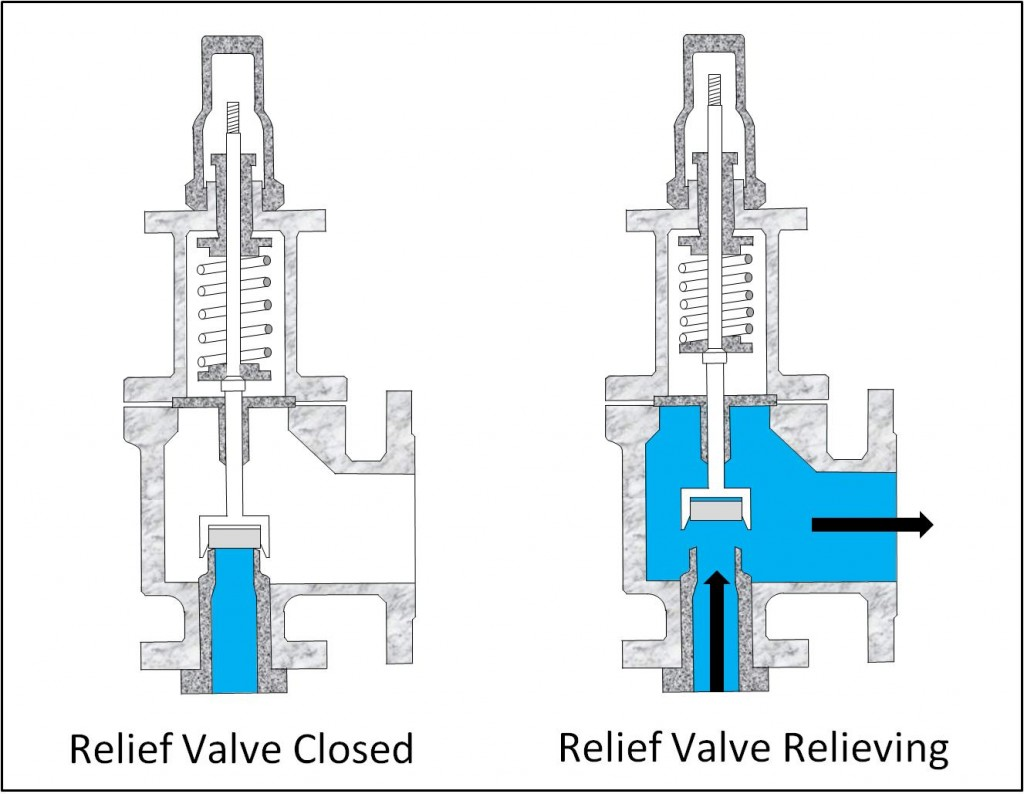
\includegraphics[scale=0.2]{media/safety-valve.jpg}
	\caption{Principe de fonctionnement d'une PSV.}
	\label{fig:safety-valve}
\end{figure}

\paragraph{Disque de rupture}
Un disque de rupture est aussi un dispositif
permettant de diminuer la pression en cas d'excès.
Il est constitué d'une membrane conçue pour céder
au-delà d'une certaine pression 
(voir figure \ref{fig:rupture-disc}). Un disque
de rupture est donc à usage unique (donc permet juste
d'évacuer la pression, pas de la réguler) et n'est pas
réglable (contrairement aux PSV) mais n'est pas
très cher et ne peut pas s'encrasser.

\begin{figure}[ht]
	\centering
	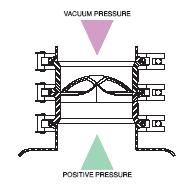
\includegraphics[scale=0.8]{media/rupture-disc.jpg}
	\caption{Principe de fonctionnement d'un disque de rupture.}
	\label{fig:rupture-disc}
\end{figure}

Comme dit précédemment, il est possible de combiner
PSV et disques de ruptures. Cela consiste à
placer un disque de rupture à l'entrée de la PSV
afin que celle-ci ne soit en contact avec les élements
chimiques que lorsque la pression est trop haute. Le
disque de rupture protège alors chimiquement le PDV et
limite la corrosion.

\subsection{Principe d'un échangeur de chaleur}
Un échangeur de chaleur est un dispositif permettant
de transférer de l'énergie thermique d'un fluide
vers un autre, sans les mélanger. Le flux thermique
traverse la surface d'échange qui sépare les fluides.
Le composant 124-MC rencontré dans la tâche 4 est un
échangeur de chaleur.

\subsection{Notions de sécurités industrielle}
Voir analyse HAZOP.

\section{Connaissance du procédé de synthèse de l'ammoniac}
\subsection{Etapes principales du procédé (tel que schématisé dans la tâche 1)}
\subsection{Fonctionnement du réacteur de synthèse} 
\subsection{Principe du recyclage de réactifs et de la purge}
\subsection{Points principaux de production et de consommation d'énergie du procédé}
\subsection{Principaux risques pour la santé et l'environnement liés aux réactifs et produits}

\section{Laboratoire d'électrolyse de l'eau}

\section{Questions de réflexion sur les thématiques traitées
dans le cadre du projet}
\subsection{Compréhension globale des impacts du procédé de l'ammoniac sur l'environnement}
\subsection{Compréhension globale des stratégies mises en place pour limiter la consommation 
énergétique sur un site de production d'ammoniac tel celui de Yara}

\end{document}